\documentclass[9pt]{ctexbeamer}

\usepackage{pgfpages}
\usepackage{tikz}

\makeatletter
\def\beamer@framenotesbegin{% at beginning of slide
	\usebeamercolor[fg]{normal text}
}
\makeatother
%%%%%%%%%%%%%%%%%%

%%%%-----导入宏包-----%%%%
\usepackage{style/shubeamer}   % SHU 主题（含配色、帧标题、页脚、Python 代码样式）
\usepackage{amsmath,amsfonts,amssymb,bm}
\usepackage{graphicx,hyperref,url}
\usepackage{comment}
\usepackage{subcaption}
\usepackage{booktabs}
\usepackage{graphbox}
\usepackage{arydshln}
\usepackage[super,square]{natbib}
\usepackage{wrapfig} % 文字绕排
\usepackage{calligra}
%%%%%%%%%%%%%%%%%%

%%%%-----设置字体-----%%%%
\setmainfont{CMU Serif}
\setsansfont{CMU Sans Serif}
%%%%%%%%%%%%%%%%%%

\definecolor{nvidia}{RGB}{102,156,28}
\definecolor{red}{RGB}{184,13,73}
\definecolor{darkred}{RGB}{145,12,7}
\definecolor{orange}{RGB}{242,151,36}
\definecolor{darkteal}{RGB}{43,106,108}
\definecolor{darkgrey}{RGB}{64,64,64}
\definecolor{darkblue}{RGB}{4,37,58}
\definecolor{tan}{RGB}{225,221,191}
\definecolor{green}{RGB}{76,131,122}
\definecolor{darkgreen}{RGB}{42,50,46}
\definecolor{bluegray}{RGB}{33,36,39}
\definecolor{brown}{RGB}{110,54,42}

% 设置 Beamer 主题
\beamertemplateballitem
\AtBeginSection[]
{
	\begin{frame}<beamer>
		\frametitle{\textbf{目录}}
		\textbf{\tableofcontents[currentsection]}
	\end{frame}
}
%%%%%%%%%%%%%%%%%%



%%%%----设定图片存放路径
\graphicspath{{figures/}}

%%%%----首页信息设置----%%%% 方括号内容将显示在页脚
\AtBeginDocument{%
	%%%%----标题
	\title[Python金融数据分析]{\fontsize{16pt}{22pt}\selectfont {Python金融数据分析}}
	%%%%----副标题
	\subtitle{\fontsize{9pt}{14pt}\selectfont \textit{工具篇：AI 辅助编程与项目版本管理}}
	%%%%----个人信息设置
	\author[王伟冠, 吕文俊]{%
		\begin{tabular}{ll}%
			主讲人： & 王伟冠, 吕文俊\tabularnewline%
			院\quad 系：   & 经济学院金融系\tabularnewline
			% \tabularnewline%
		\end{tabular}
	}
	%%%%----机构信息
	\institute[SHU]{上海大学}
	%%%%----日期信息
	\date[\today]{\today}}
%%%%----Macros for Vector, Matrix, Tensor, Math Operator and Misc
\input{style/macros.tex}
%%%%%%%%%%%%%%%%%%



\begin{document}

%% 封面信息，方括号内容是显示在页脚的短标题
\begin{frame}
	\titlepage
\end{frame}

%% 提纲页
\section*{目录}
\label{sec:toc}

\begin{frame}
	\frametitle{\textbf{目录}}
	\textbf{\tableofcontents}
\end{frame}


\section{工具分工与项目流程}

\begin{frame}{本章目标：把一次分析做成可检查的项目}
  \begin{tabular}{p{0.22\textwidth}p{0.66\textwidth}}
    \toprule
    工具 & 在课程中的分工 \\
    \midrule
    VS Code & 查看和编辑文件，运行脚本与 Notebook。\\[7pt]
    Python 与 uv & 执行代码，管理项目的解释器与依赖。\\[7pt]
    Qoder & 根据任务读取项目，辅助编写、修改和验证代码。\\[7pt]
    Git & 比较修改，记录版本，在分支中尝试新方案。\\
    \bottomrule
  \end{tabular}
  \begin{block}{贯穿全章的工作流程}
    建立项目 $\rightarrow$ 提出任务 $\rightarrow$ 检查修改与结果 $\rightarrow$ 保存版本。
  \end{block}
  第一章讨论学习目标；本工具篇准备工作环境；后续章节学习 Python 与数据分析。
\end{frame}

\begin{frame}{看图认识 VS Code：文件、代码与终端在哪里？}
  \begin{columns}[T,totalwidth=\textwidth]
    \begin{column}{0.70\textwidth}
      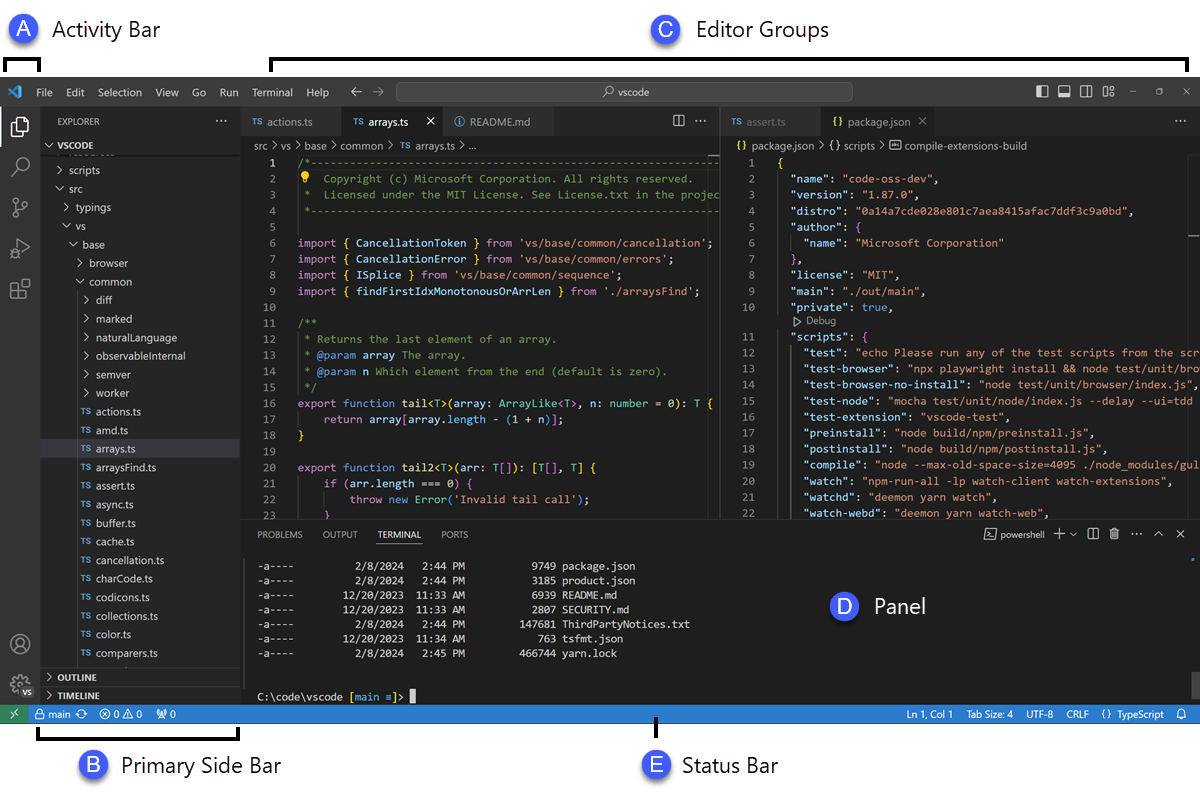
\includegraphics[width=\linewidth]{vscode-interface.png}
    \end{column}
    \begin{column}{0.28\textwidth}
      \small
      \textbf{A 活动栏}\\切换文件、搜索、Git 等视图。\par\medskip
      \textbf{B 侧边栏}\\展开项目目录，找到代码文件。\par\medskip
      \textbf{C 编辑区}\\阅读和修改代码。\par\medskip
      \textbf{D 面板}\\打开终端，执行项目命令。\par\medskip
      \textbf{E 状态栏}\\查看分支等当前状态。
    \end{column}
  \end{columns}
  \begin{block}{课堂操作}
    用“文件 $\rightarrow$ 打开文件夹”打开 \texttt{py4fi-course}，在侧边栏找到环境文件。
  \end{block}
  {\tiny 图片：\href{https://code.visualstudio.com/docs/editing/getting-started/userinterface}{VS Code 官方界面指南}；图中为官方示例项目，字母对应右侧中文说明。}
\end{frame}

\section{虚拟环境搭建}

\begin{frame}{为什么要使用虚拟环境？}
  \begin{block}{同一台电脑，两个金融分析项目}
    旧项目依赖 pandas 旧版接口，新项目需要新版功能。\par
    如果共用一套包，升级新项目的依赖可能让旧代码无法运行。
  \end{block}
  \begin{columns}[T,totalwidth=\textwidth]
    \begin{column}{0.48\textwidth}
      \begin{block}{项目 A：历史回测}
        项目 A 的代码\\
        项目 A 的 \texttt{.venv}\\
        适合旧代码的 Python 与包版本
      \end{block}
    \end{column}
    \begin{column}{0.48\textwidth}
      \begin{block}{项目 B：新数据分析}
        项目 B 的代码\\
        项目 B 的 \texttt{.venv}\\
        适合新代码的 Python 与包版本
      \end{block}
    \end{column}
  \end{columns}
  \begin{itemize}
    \item \textbf{隔离依赖}：各项目分别安装包，减少版本冲突。
    \item \textbf{方便复现}：记录 Python 与依赖版本，在其他电脑上重建环境。
    \item \texttt{.venv} 是项目中的一个文件夹；代码和数据放在它的外面。
  \end{itemize}
\end{frame}

\begin{frame}{虚拟环境背后的简要机制}
  \centering
  \begin{tikzpicture}[
    box/.style={draw=shublue, fill=shulight, rounded corners=3pt,
      text width=2.65cm, minimum height=1.35cm, align=center, font=\small},
    arr/.style={->, >=stealth, thick, draw=shublue}]
    \node[box] (code) at (0,0) {项目代码\\\texttt{import pandas}};
    \node[box] (python) at (3.6,0) {选中的 Python 解释器\\\texttt{.venv} 中的入口};
    \node[box] (packages) at (7.2,0) {该环境的第三方包\\\texttt{site-packages}};
    \draw[arr] (code) -- (python);
    \draw[arr] (python) -- (packages);
  \end{tikzpicture}
  \vspace{0.4cm}
  \begin{itemize}
    \item 创建环境时，工具配置 Python 入口、环境配置和独立的包目录。
    \item 该入口关联一个基础 Python 安装；运行时识别环境位置，使用对应的包搜索路径，默认不包含系统的第三方包目录。
    \item \texttt{.venv/pyvenv.cfg} 记录基础 Python 等环境信息。
    \item 激活环境会把其命令目录放到当前终端的 \texttt{PATH} 前面，使输入 \texttt{python} 时优先找到它。
  \end{itemize}
  \begin{block}{关键区别}
    虚拟环境隔离 Python 包；它不创建新的操作系统，也不是虚拟机。
  \end{block}
  {\tiny\href{https://docs.python.org/3/library/venv.html}{机制参考：Python 官方 venv 文档}}
\end{frame}

\begin{frame}{工具分工：本课程使用 uv}
  \begin{tabular}{p{0.17\textwidth}p{0.72\textwidth}}
    \toprule
    工具 & 主要用途 \\
    \midrule
    Python & 解释并执行我们的代码。\\[5pt]
    venv & Python 自带的虚拟环境创建工具，通常搭配 pip 装包。\\[5pt]
    conda & 管理环境与包，也能处理许多非 Python 依赖。\\[5pt]
    uv & 管理 Python 版本、创建虚拟环境、安装包并记录项目依赖。\\
    \bottomrule
  \end{tabular}
  \vspace{0.35cm}
  \begin{block}{从零搭建的顺序}
    安装 uv $\rightarrow$ 新建项目 $\rightarrow$ 创建 \texttt{.venv}
    $\rightarrow$ 安装分析包 $\rightarrow$ 运行并检查 $\rightarrow$ 保存环境说明文件。
  \end{block}
  \begin{itemize}
    \item 本次练习从个人目录中的\textbf{全新文件夹}开始，无需现成环境文件。
    \item Windows 使用 \textbf{PowerShell}；macOS 使用\textbf{终端（zsh）}。
    \item 标注“两系统相同”的命令，在两种终端中都可直接运行。
  \end{itemize}
\end{frame}

\begin{frame}[fragile]{第一步：安装 uv（Windows / macOS）}
  \textbf{Windows：打开 PowerShell}
\begin{lstlisting}[language={},numbers=none,basicstyle=\ttfamily\scriptsize]
powershell -ExecutionPolicy ByPass -c "irm https://astral.sh/uv/install.ps1 | iex"
\end{lstlisting}
  \textbf{macOS：打开终端}
\begin{lstlisting}[language={},numbers=none]
curl -LsSf https://astral.sh/uv/install.sh | sh
\end{lstlisting}
  \textbf{安装完成后，关闭并重新打开终端；两系统相同：}
\begin{lstlisting}[language={},numbers=none]
uv --version
\end{lstlisting}
  \begin{itemize}
    \item 显示 uv 的版本号，说明终端已经能找到 uv 命令。
    \item 此时安装的是\textbf{环境管理工具}；分析用的包稍后再安装。
    \item 无需提前安装 Python；后续创建环境时，uv 可下载缺少的 Python。
  \end{itemize}
  {\tiny\href{https://docs.astral.sh/uv/getting-started/installation/}{命令来源：uv 官方安装文档}}
\end{frame}

\begin{frame}[fragile]{第二步：从空文件夹开始创建项目}
  \begin{columns}[T,totalwidth=\textwidth]
    \begin{column}{0.48\textwidth}
      \textbf{Windows / PowerShell}
\begin{lstlisting}[language={},numbers=none]
cd $HOME
mkdir py4fi-course
cd py4fi-course
\end{lstlisting}
    \end{column}
    \begin{column}{0.48\textwidth}
      \textbf{macOS / 终端}
\begin{lstlisting}[language={},numbers=none]
cd ~
mkdir py4fi-course
cd py4fi-course
\end{lstlisting}
    \end{column}
  \end{columns}
  \textbf{以下命令两系统相同：}
\begin{lstlisting}[language={},numbers=none]
uv init --bare --python 3.11
uv python pin 3.11
\end{lstlisting}
  \begin{itemize}
    \item \texttt{mkdir} 创建文件夹，\texttt{cd} 进入文件夹；后续命令都在这里执行。
    \item \texttt{uv init --bare} 创建最小的 \texttt{pyproject.toml}，初始依赖为空。
    \item \texttt{uv python pin} 把项目选用的 Python 版本写入 \texttt{.python-version}。
    \item 这一步是在写项目说明，\textbf{还没有安装分析包}。
  \end{itemize}
\end{frame}

\begin{frame}[fragile]{第三步：创建虚拟环境，检查 Python 的位置}
  \textbf{Windows / macOS 相同：在 py4fi-course 文件夹中运行}
\begin{lstlisting}[language={},numbers=none]
uv venv --python 3.11 --prompt py4fi-course
\end{lstlisting}
  \begin{itemize}
    \item uv 找到或下载 Python 3.11，再创建当前项目的 \texttt{.venv} 文件夹。
    \item \texttt{--prompt py4fi-course} 设置激活后的显示名称；环境目录仍是 \texttt{.venv}，分析包稍后安装。
  \end{itemize}
  \textbf{直接调用环境中的 Python，无需先激活：}
  \begin{columns}[T,totalwidth=\textwidth]
    \begin{column}{0.48\textwidth}
      Windows / PowerShell
\begin{lstlisting}[language={},numbers=none,basicstyle=\ttfamily\scriptsize]
.\.venv\Scripts\python.exe -c "import sys; print(sys.executable)"
\end{lstlisting}
    \end{column}
    \begin{column}{0.48\textwidth}
      macOS / 终端
\begin{lstlisting}[language={},numbers=none,basicstyle=\ttfamily\scriptsize]
./.venv/bin/python -c "import sys; print(sys.executable)"
\end{lstlisting}
    \end{column}
  \end{columns}
  \begin{block}{观察结果}
    输出路径应位于 \texttt{py4fi-course} 的 \texttt{.venv} 中。\par
    Windows 的命令目录叫 \texttt{Scripts}，macOS 的叫 \texttt{bin}。
  \end{block}
\end{frame}

\begin{frame}[fragile]{第四步：安装分析包，并完成一次验证}
  \textbf{Windows / macOS 相同：}
\begin{lstlisting}[language={},numbers=none]
uv add numpy "pandas>=2.2,<3.0" matplotlib
uv add jupyterlab ipykernel
uv pip list
uv run python -c "import pandas as pd; print(pd.__version__)"
\end{lstlisting}
  \begin{itemize}
    \item 前三个包用于数值计算、表格分析和绘图；后两个支持 Notebook。
    \item pandas 限定为 2.x，以配合课程现有代码；引号让终端完整传入版本条件。
    \item \texttt{uv add} 把需求写入 \texttt{pyproject.toml}，解析兼容版本，生成或更新 \texttt{uv.lock}，并安装到 \texttt{.venv}。
    \item 包还会依赖其他包，因此 \texttt{uv pip list} 通常比手动添加的名单长。
  \end{itemize}
  \begin{block}{怎样判断成功？}
    最后一行能导入 pandas 并显示版本号；上一页已确认解释器位置。
  \end{block}
\end{frame}

\begin{frame}[fragile]{环境文件（一）：读懂 pyproject.toml}
  \textbf{示意片段：描述项目需要什么，具体下限可能因安装时间不同而变化。}
\begin{lstlisting}[language={},numbers=none]
[project]
name = "py4fi-course"
version = "0.1.0"
requires-python = ">=3.11"
dependencies = [
    "numpy>=2.0",
    "pandas>=2.2,<3.0",
    "matplotlib>=3.9",
]
\end{lstlisting}
  \begin{itemize}
    \item \texttt{name}、\texttt{version} 是\textbf{项目}的名称和版本，不是 Python 版本。
    \item \texttt{requires-python} 是允许的 Python 范围；\texttt{.python-version} 指定本项目选用的版本，如 \texttt{3.11}。
    \item \texttt{dependencies} 是直接依赖；\texttt{>=} 为最低版本，\texttt{<} 为上限，\texttt{==} 为固定版本。
    \item 日常用 \texttt{uv add} 修改依赖；这个文件本身不包含 Python 或包代码。
  \end{itemize}
\end{frame}

\begin{frame}{环境文件（二）：说明文件和实际环境有什么区别？}
  \small
  \begin{tabular}{p{0.23\textwidth}p{0.43\textwidth}p{0.22\textwidth}}
    \toprule
    文件或目录 & 保存什么 & 如何管理 \\
    \midrule
    \texttt{pyproject.toml} & 项目信息、Python 范围、直接依赖要求 & 随项目保存 \\[7pt]
    \texttt{.python-version} & 选用的 Python 版本，如 3.11 & 随项目保存 \\[7pt]
    \texttt{uv.lock} & 解析后的准确包版本及间接依赖；可含不同平台的条件 & 随项目保存，由 uv 更新 \\[7pt]
    \texttt{.venv/} & 本机实际使用的 Python 入口、配置和已安装包 & 本机生成，不跨电脑复制 \\[7pt]
    \texttt{requirements.txt} & 另一种常见依赖清单，可写版本约束；内容不一定完整锁定 & 本流程无需额外创建 \\
    \bottomrule
  \end{tabular}
  \vspace{0.3cm}
  \begin{block}{从需求到安装结果}
    \texttt{pyproject.toml}（要求）$\rightarrow$ \texttt{uv.lock}（解析结果）
    $\rightarrow$ \texttt{.venv}（本机环境）。\par
    环境文件用于\textbf{重建}环境；它们不等于环境本身。
  \end{block}
  {\tiny\href{https://docs.astral.sh/uv/guides/projects/}{参考：uv 项目结构与依赖管理}}
\end{frame}

\begin{frame}[fragile]{第五步：日常运行与“激活”的含义}
  \textbf{推荐方式：在项目文件夹内运行；Windows / macOS 相同}
\begin{lstlisting}[language={},numbers=none]
uv run jupyter lab
uv run python analysis.py
\end{lstlisting}
  {\small 第一行启动 JupyterLab；第二行用于运行自己已保存的 \texttt{analysis.py}。\par
  \texttt{uv run} 会检查项目环境并在需要时同步依赖，再执行命令，无需手动激活。\par}
  \vspace{0.15cm}
  \textbf{也可以手动激活，再直接输入 python：}
  \begin{columns}[T,totalwidth=\textwidth]
    \begin{column}{0.48\textwidth}
      Windows / PowerShell
\begin{lstlisting}[language={},numbers=none]
.\.venv\Scripts\Activate.ps1
python --version
deactivate
\end{lstlisting}
    \end{column}
    \begin{column}{0.48\textwidth}
      macOS / 终端
\begin{lstlisting}[language={},numbers=none]
source .venv/bin/activate
python --version
deactivate
\end{lstlisting}
    \end{column}
  \end{columns}
  \begin{itemize}
    \item 激活只影响当前终端的命令查找；\texttt{deactivate} 恢复，不会删除环境。
    \item PowerShell 若限制激活脚本，直接使用上方的 \texttt{uv run} 即可。
  \end{itemize}
\end{frame}

\begin{frame}[fragile]{第六步：在 VS Code 中选对 Notebook 内核}
  \begin{enumerate}
    \item 用 VS Code 打开 \texttt{py4fi-course} 文件夹，安装 Microsoft 的 \textbf{Python} 和 \textbf{Jupyter} 扩展。
    \item 新建或打开 \texttt{.ipynb} 文件，点击右上角 \textbf{Select Kernel}，从 Python 环境中选择本项目的 \texttt{.venv}。
  \end{enumerate}
  \begin{block}{对应的解释器路径}
    Windows：\texttt{py4fi-course\textbackslash .venv\textbackslash Scripts\textbackslash python.exe}\par
    macOS：\texttt{py4fi-course/.venv/bin/python}
  \end{block}
  \textbf{在 Notebook 单元格运行，两系统相同：}
\begin{lstlisting}[language=Python,numbers=none]
import sys
import pandas as pd
print(sys.executable)
print(pd.Series([0.01, -0.02, 0.03]).mean())
\end{lstlisting}
  {\small 路径应指向项目的 \texttt{.venv}，平均收益率约为 \texttt{0.00667}。\par
  若提示找不到包：先核对内核路径，再在项目终端运行 \texttt{uv add 包名}。\par
  终端激活环境，并不自动替换 Notebook 已选的内核。}
  \par{\tiny\href{https://code.visualstudio.com/docs/datascience/jupyter-notebooks}{参考：VS Code 官方 Notebook 指南}}
\end{frame}

\begin{frame}{看图选择 Notebook 内核：认路径，再选环境}
  \textbf{1. 点击 Notebook 右上角的 Select Kernel，打开内核选择器。}\par\medskip
  {\centering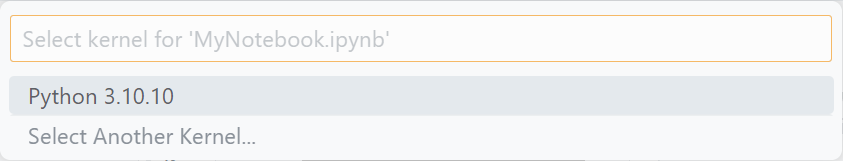
\includegraphics[width=0.65\linewidth]{vscode-kernel.png}\par}
  {\small 若列表只有最近用过的环境，选择 \textbf{Select Another Kernel...}，再查看 Python 环境。}\par\medskip
  \textbf{2. 对照环境路径，找到当前项目的 .venv。}\par\medskip
  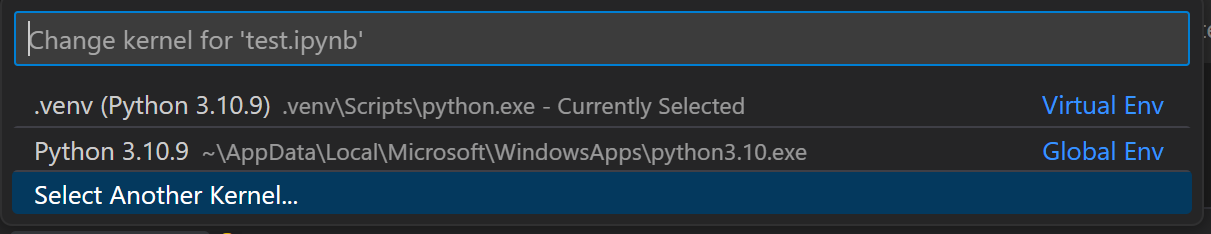
\includegraphics[width=\linewidth]{vscode-notebook.png}
  \begin{block}{本课程要核对什么？}
    图中 \texttt{.venv\textbackslash Scripts\textbackslash python.exe} 是虚拟环境入口；全局环境另列一行。\par
    图示版本为 3.10；课堂应选择自己创建的 Python 3.11 环境，并运行 \texttt{sys.executable} 核对路径。
  \end{block}
  {\tiny 图片：\href{https://code.visualstudio.com/docs/datascience/jupyter-kernel-management}{VS Code 内核管理}与\href{https://code.visualstudio.com/docs/datascience/jupyter-notebooks}{Notebook 指南}；不同版本的菜单外观可能不同。}
\end{frame}

\begin{frame}[fragile]{最后：把自己搭建的环境交给另一台电脑}
  \begin{enumerate}
    \item 保存代码、数据说明及三个文件：\texttt{pyproject.toml}、\texttt{uv.lock}、\texttt{.python-version}。\textbf{不复制 .venv 文件夹。}
    \item 在另一台电脑安装 uv，进入收到的项目文件夹。
    \item 用保存的依赖记录重建，并检查运行结果。
  \end{enumerate}
  \textbf{Windows / macOS 相同：}
\begin{lstlisting}[language={},numbers=none]
uv sync --locked
uv run python -c "import sys; print(sys.executable)"
uv run python -c "import pandas as pd; print(pd.__version__)"
\end{lstlisting}
  \begin{itemize}
    \item \texttt{uv sync --locked} 按已有锁定文件同步环境；如果声明与锁文件不一致，会提示错误，需先由项目维护者更新锁文件。
    \item Windows 与 macOS 的环境目录结构和安装文件可能不同，应分别重建。
    \item 复现包版本是基础；分析结果还取决于数据、随机种子及运行平台等。
  \end{itemize}
  \begin{block}{课堂回顾}
    先亲手创建环境和添加依赖，再理解：课程提供的环境文件，就是这些步骤留下的可复用记录。
  \end{block}
\end{frame}

\section{AI 辅助编程：以 Qoder 为例}

\begin{frame}{认识 Qoder：围绕项目完成编程任务}
  \begin{itemize}
    \item 在 Qoder 中打开本地项目，说明需要完成的任务和涉及的文件。
    \item 让 AI 辅助阅读代码、保存修改、执行命令，并报告运行结果。
    \item 在 VS Code 中阅读代码、运行 Notebook，核对计算和输出。
  \end{itemize}
  \begin{block}{本章统一使用 Qoder 示例}
    本章使用 Qoder CN 桌面端；同类工具可沿用相同的任务描述与验证流程。
  \end{block}
  \begin{block}{一次任务的交付物}
    修改后的项目文件、实际运行结果，以及对修改内容的解释。
  \end{block}
  {\tiny\href{https://docs.qoder.cn/qoder/quickstart}{参考：Qoder CN 官方快速入门}}
\end{frame}

\begin{frame}{AI 编程：模型、上下文与工具}
  \begin{block}{AI 编程是什么？}
    用自然语言描述需求，让 AI 辅助编写、解释和修改代码，\par
    再通过实际运行与结果检查，逐步完成任务。
  \end{block}
  \begin{tabular}{p{0.18\textwidth}p{0.71\textwidth}}
    \toprule
    组成 & 在课程项目中的作用 \\
    \midrule
    大语言模型 & 根据需求与已有信息，生成代码和解释。\\[7pt]
    项目上下文 & 提供当前代码、数据字段、报错和环境信息。\\[7pt]
    工具 & 在授权范围内读取文件、保存修改、执行命令。\\
    \bottomrule
  \end{tabular}
  \vspace{0.2cm}
  \begin{itemize}
    \item 编程智能体（Agent）把模型与工具结合，按任务需要反复执行和调整。
    \item 回复中的代码要经过运行；程序能运行，还要检查公式和数据口径。
    \item 学习时请 AI 解释关键步骤，并尝试自己修改输入、预测输出。
  \end{itemize}
  {\tiny\href{https://docs.qoder.cn/qoder/quickstart}{软件操作参考：Qoder CN 官方快速入门}}
\end{frame}

\begin{frame}{打开 Qoder，并关联课程项目}
  \begin{enumerate}
    \item 从 \href{https://qoder.cn/download}{Qoder CN 官方下载页}安装桌面端并登录。
    \item 选择\textbf{编程}，将前面创建的 \texttt{py4fi-course} 文件夹添加为工作区。
    \item 选择\textbf{本地模式}，确认工作区完整路径与当前分支，再开始新任务。
    \item 在 VS Code 中打开同一个目录，选好 \texttt{.venv} 解释器或 Notebook 内核。
    \item 先发送一个阅读任务：“列出本项目的环境文件，解释它们的作用，暂不修改文件。”
  \end{enumerate}
  \begin{block}{两个窗口，一份项目文件}
    对照两边的完整路径；确认 Qoder 读取的文件就是 VS Code 中的文件。
  \end{block}
  {\small 桌面端入口名称可能随版本变化；以官方指南和当前界面为准。}
  \par{\tiny\href{https://docs.qoder.cn/qoder/quickstart}{参考：Qoder CN 官方快速入门}}
\end{frame}

\begin{frame}{协作流程：提出需求、查看修改、运行验证}
  \centering
  \begin{tikzpicture}[
    workflowstage/.style={draw, rounded corners=3pt, text width=2.6cm,
      minimum height=1.7cm, align=center, font=\small, inner sep=6pt},
    arr/.style={->, >=stealth, thick, draw=shublue}]
    \node[workflowstage,draw=shugold,fill=shugold!12] (human) at (0,0)
      {\textbf{1. 人明确任务}\\[5pt]分析目标与数据\\允许修改的文件\\预期输出与判断标准};
    \node[workflowstage,draw=shusky,fill=shusky!10] (ai) at (3.65,0)
      {\textbf{2. Qoder 执行}\\[5pt]读取项目上下文\\生成或修改代码\\说明修改及运行情况};
    \node[workflowstage,draw=shugold,fill=shugold!12] (review) at (7.3,0)
      {\textbf{3. 人验证结果}\\[5pt]阅读代码与变更\\使用项目环境运行\\核对输出与金融含义};
    \draw[arr] (human) -- (ai);
    \draw[arr] (ai) -- (review);
    \draw[arr] (review.south) -- ++(0,-0.55) -|
      node[pos=0.25,below,font=\footnotesize,text=shugray]
      {把具体报错或差异反馈给 AI，修改后再次验证} (human.south);
  \end{tikzpicture}
  \vspace{0.4cm}
  \begin{block}{向 AI 交代环境和边界}
    使用本项目的 \texttt{.venv}；先说明修改方案；保留已有编辑；\par
    修改后列出变更文件、执行的命令，以及仍需我确认的结果。
  \end{block}
  \begin{itemize}
    \item 交给 AI 修改前，先保存 VS Code 中的编辑；同一文件避免同时修改。
    \item AI 完成后查看磁盘上的最新内容；不要用未保存的旧内容覆盖新修改。
    \item 人负责核对数据、公式与经济解释，AI 的完成提示是验证的起点。
  \end{itemize}
\end{frame}

\begin{frame}{向 AI 描述任务：目标、输入、约束、验收}
  \begin{block}{课堂提示词示例：在桌面端关联 py4fi-course 后输入}
    请新建 \texttt{returns\_demo.py}，计算价格序列
    \texttt{[100, 110, 99]} 的两期简单收益率和累计收益率。\par\medskip
    仅使用 Python 标准库；用本项目的 \texttt{.venv} 运行；
    不修改其他文件。先解释公式，再编写和运行代码。\par\medskip
    输出两期收益率和累计收益率，保留两位小数并显示百分号；
    列出运行命令，解释累计收益率为什么不等于两期收益率之和。
  \end{block}
  \begin{itemize}
    \item \textbf{目标与输入}：指定计算任务与完整的示例数据。
    \item \textbf{约束}：说明文件范围、Python 环境和可用依赖。
    \item \textbf{验收}：明确输出格式、运行证据和需要解释的问题。
    \item 若结果有误，反馈实际输出与预期差异；若报错，附完整报错。
  \end{itemize}
\end{frame}

\begin{frame}[fragile]{课堂验证：两期收益率如何累计？}
  \textbf{在 VS Code 阅读 AI 生成的文件，并与下面的计算核对：}
\begin{lstlisting}[language=Python,numbers=none]
prices = [100, 110, 99]
r1 = prices[1] / prices[0] - 1
r2 = prices[2] / prices[1] - 1
total = (1 + r1) * (1 + r2) - 1
print(f"Period 1: {r1:.2%}")
print(f"Period 2: {r2:.2%}")
print(f"Total: {total:.2%}")
\end{lstlisting}
  \begin{block}{手算验收}
    两期收益率为 $+10\%$ 和 $-10\%$；累计收益率为\par
    $(1+10\%)(1-10\%)-1=-1\%$，也等于 $99/100-1$。
  \end{block}
  \begin{itemize}
    \item 在项目目录运行 \texttt{uv run python returns\_demo.py}，核对三个输出。
    \item 两期简单收益率直接相加得到 $0\%$，不代表持有期累计收益率。
    \item 将末期价格改成 100，先预测再运行：累计收益率应为 $0\%$。
  \end{itemize}
\end{frame}

\section{Git 版本管理与 Agent 协作}

\begin{frame}{Git 是什么，可以做什么？}
  \begin{block}{为项目记录可以追溯的版本}
    Git 是分布式版本控制工具。每次提交（commit）记录一个项目快照，
    并保存作者、时间、说明和版本之间的关系。
  \end{block}
  \begin{itemize}
    \item \textbf{比较修改}：Agent 改了哪些文件、哪些行，计算逻辑是否改变？
    \item \textbf{查阅历史}：哪个版本能运行？某个公式为什么被修改？
    \item \textbf{尝试新方案}：在分支上实验，验证后再合并到主线。
    \item \textbf{恢复与协作}：找回已记录的内容，与他人交换已提交的版本。
  \end{itemize}
  \begin{block}{本课程中的例子}
    为 \texttt{returns\_demo.py} 记录“完成两期收益率计算”，
    再记录“支持任意长度价格序列”，无需保存多个“最终版”文件。
  \end{block}
  {\tiny\href{https://git-scm.com/docs/gittutorial}{参考：Git 官方入门教程}}
\end{frame}

\begin{frame}{Git 如何工作：工作区、暂存区、仓库}
  \centering
  \begin{tikzpicture}[
    box/.style={draw=shublue,fill=shulight,rounded corners=3pt,
      text width=2.6cm,minimum height=1.7cm,align=center,font=\small},
    arr/.style={->,>=stealth,thick,draw=shublue}]
    \node[box] (work) at (0,0) {\textbf{工作区}\\[6pt]磁盘上的项目文件\\你与 Agent 在这里编辑};
    \node[box] (stage) at (3.65,0) {\textbf{暂存区}\\[6pt]选入下一次提交的内容\\可以只选部分文件};
    \node[box] (repo) at (7.3,0) {\textbf{本地仓库}\\[6pt]已经提交的版本历史\\通常存放在 \texttt{.git}};
    \draw[arr] (work) -- node[above,font=\scriptsize]{\texttt{git add}} (stage);
    \draw[arr] (stage) -- node[above,font=\scriptsize]{\texttt{git commit}} (repo);
  \end{tikzpicture}
  \vspace{0.4cm}
  \begin{itemize}
    \item \textbf{保存文件}更新工作区；\textbf{add}选取内容；\textbf{commit}记录版本。
    \item 暂存的是执行 add 时的内容；随后又改了文件，需要再次 add。
    \item 提交在本地完成，无需联网；\textbf{push}才把提交发送到远程仓库。
    \item Git 不会自动记录每次编辑；没有提交的内容不属于已保存的版本历史。
  \end{itemize}
  {\tiny\href{https://git-scm.com/docs/git-add}{参考：git add}\quad
  \href{https://git-scm.com/docs/git-push}{git push}}
\end{frame}

\begin{frame}[fragile]{第一步：准备 Git 并创建仓库}
  \begin{enumerate}
    \item 从 \href{https://git-scm.com/install/}{\textbf{git-scm.com/install}} 按系统说明安装 Git，重新打开终端。
    \item 进入前面创建的 \texttt{py4fi-course} 文件夹，执行下列命令。
  \end{enumerate}
\begin{lstlisting}[language={},numbers=none]
git --version
git init -b main
git config user.name "Your Name"
git config user.email "you@example.com"
git status
\end{lstlisting}
  \begin{itemize}
    \item \texttt{init} 创建本地仓库，\texttt{main} 是本练习的主分支名称。
    \item 把示例姓名和邮箱换成自己的；此处配置只作用于当前仓库。
    \item 姓名与邮箱用于标注提交作者，不是 GitHub 的登录信息。
    \item 若 uv 已创建 Git 仓库，跳过 init；用 \texttt{git branch --show-current} 查看当前分支名，后续按实际名称操作。
  \end{itemize}
  {\tiny\href{https://git-scm.com/docs/gittutorial}{参考：Git 初始化与作者配置}}
\end{frame}

\begin{frame}[fragile]{第二步：选择要记录的文件}
  \textbf{在项目根目录创建或补充 .gitignore，每行一个忽略规则：}
\begin{lstlisting}[language={},numbers=none]
.venv/
__pycache__/
.ipynb_checkpoints/
.env
data/raw/
\end{lstlisting}
  \begin{itemize}
    \item \textbf{提交}：代码、说明、\texttt{.gitignore}，以及前面生成的
      \texttt{pyproject.toml}、\texttt{uv.lock}、\texttt{.python-version}。
    \item \textbf{忽略}：本机环境、缓存、存放密钥的 \texttt{.env} 和本例的原始数据目录。
    \item 数据另行保存来源与获取说明；Notebook 提交前检查输出中的数据内容。
    \item \texttt{.gitignore} 只影响未跟踪文件，不会自动移除已经提交的文件或历史。
  \end{itemize}
  \begin{block}{添加前先看一眼}
    使用 \texttt{git status} 查看文件清单，再按文件名添加；
    忽略文件仍保留在电脑上。
  \end{block}
  {\tiny\href{https://git-scm.com/docs/gitignore}{参考：Git 忽略规则}}
\end{frame}

\begin{frame}[fragile]{第三步：记录第一个可运行版本}
  \textbf{承接收益率示例：先保存文件，再在项目目录执行。}
\begin{lstlisting}[language={},numbers=none]
uv run python returns_demo.py
git status
git add returns_demo.py .gitignore
git add pyproject.toml uv.lock .python-version
git diff --cached
git commit -m "Add two-period returns example"
git log -5 --format="%s"
\end{lstlisting}
  \begin{itemize}
    \item 核对收益率输出为 $10\%$、$-10\%$ 和 $-1\%$，再记录这一版本。
    \item \texttt{diff --cached} 展示即将提交的内容；有遗漏时补充 add。
    \item \texttt{commit -m} 写明这次做了什么；最后一行查看最近 5 次提交的标题。
    \item 如果提示 \texttt{nothing to commit}，说明当前没有可提交的新内容。
  \end{itemize}
  {\tiny\href{https://git-scm.com/docs/gittutorial}{参考：提交与查看历史}}
\end{frame}

\begin{frame}{看图理解暂存：先选文件，再记录版本}
  \begin{columns}[T,totalwidth=\textwidth]
    \begin{column}{0.49\textwidth}
      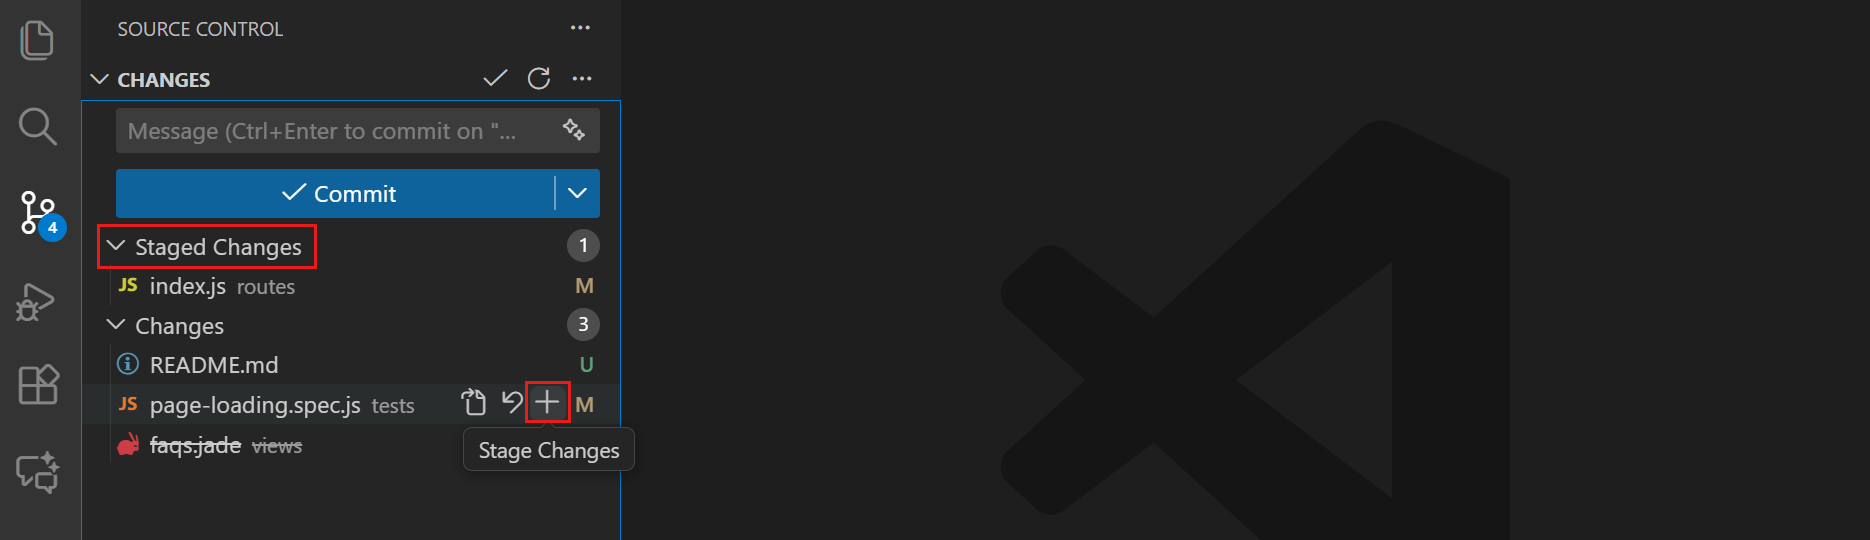
\includegraphics[width=\linewidth,trim=0 0 610 0,clip]{vscode-stage.png}
    \end{column}
    \begin{column}{0.48\textwidth}
      \small
      \textbf{Changes：尚未暂存}\\
      先点击文件查看差异，再点击该文件旁的 \textbf{+}，选入下一次提交。\par\medskip
      \textbf{Staged Changes：已经暂存}\\
      对应 \texttt{git diff --cached}；这里的内容将进入提交。\par\medskip
      \textbf{Message 与 Commit}\\
      写明本次完成的任务，核对暂存内容后提交。\par\medskip
      图中的 \textbf{M} 表示已修改，\textbf{U} 表示尚未跟踪。
    \end{column}
  \end{columns}
  \begin{block}{迁移到收益率练习}
    找到 \texttt{returns\_demo.py}，核对修改并运行，再暂存该文件；\par
    暂存后若继续编辑，需要再次暂存，才会把后续修改加入提交。
  \end{block}
  {\tiny 图片：\href{https://code.visualstudio.com/docs/sourcecontrol/staging-commits}{VS Code 官方暂存与提交指南}（仅展示左侧操作区域）；示例文件名不同，操作相同。}
\end{frame}

\begin{frame}[fragile]{日常检查：改了什么，哪些会被提交？}
\begin{lstlisting}[language={},numbers=none]
git status
git diff -- returns_demo.py
git diff --cached -- returns_demo.py
git log -5 --format="%s"
\end{lstlisting}
  \begin{itemize}
    \item \texttt{status}：区分未跟踪、未暂存、已暂存的文件。
    \item \texttt{diff}：比较工作区与暂存区；\texttt{diff --cached}：比较暂存区与上次提交。
    \item 新建且未跟踪的文件不会出现在普通 diff 中，应直接打开检查。
    \item VS Code 的\textbf{源代码管理}面板也可查看文件差异、暂存和提交。
  \end{itemize}
  \begin{block}{只想撤销暂存，保留代码修改}
    已有首次提交后，执行
    \texttt{git restore --staged returns\_demo.py}。\par
    不带 \texttt{--staged} 的 restore 会改写工作区文件，含义不同。
  \end{block}
  {\tiny\href{https://git-scm.com/docs/git-diff}{参考：git diff}\quad
  \href{https://git-scm.com/docs/git-restore}{git restore}}
\end{frame}

\begin{frame}{看图阅读 diff：这次到底改了哪些代码？}
  \begin{columns}[T,totalwidth=\textwidth]
    \begin{column}{0.72\textwidth}
      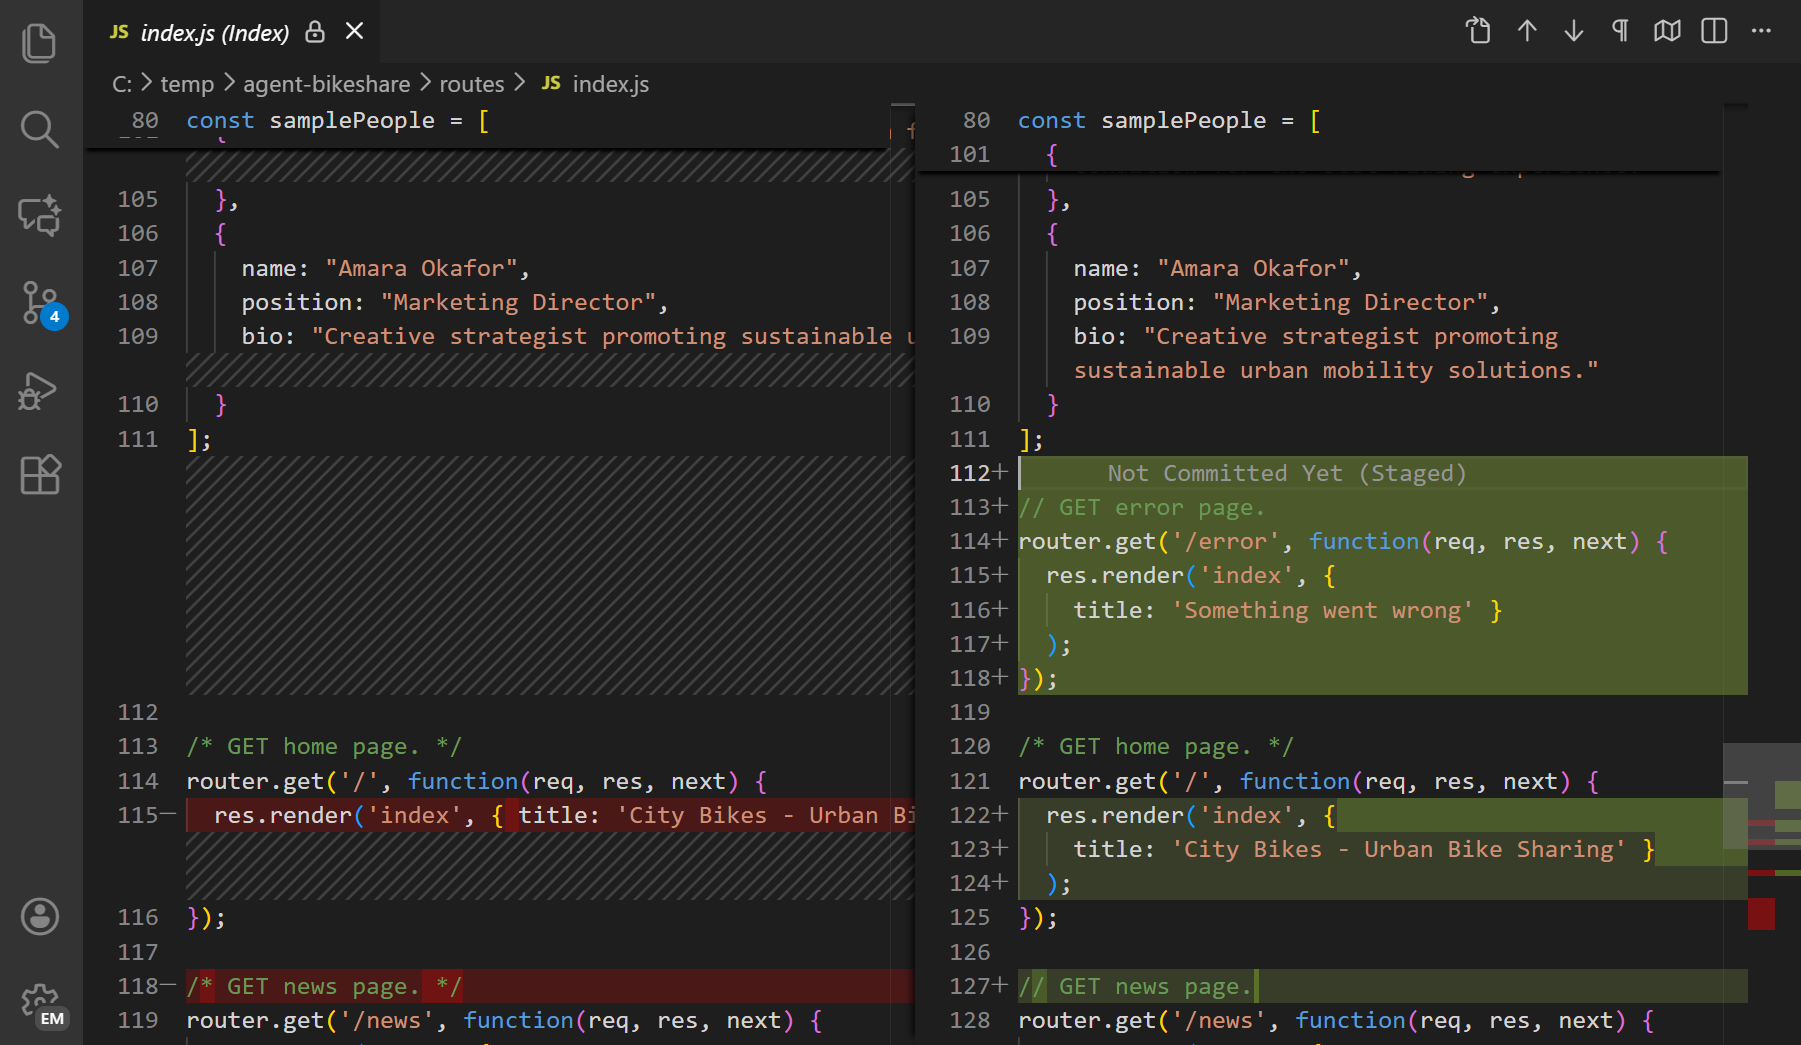
\includegraphics[width=\linewidth]{vscode-diff.png}
    \end{column}
    \begin{column}{0.25\textwidth}
      \small
      \textbf{左侧：比较基准}\\红色区域表示删去或被替换的内容。\par\medskip
      \textbf{右侧：待检查版本}\\绿色区域表示增加或替换后的内容。\par\medskip
      \textbf{先看比较对象}\\从 Changes 打开时，看未暂存修改；从 Staged Changes 打开时，看将提交的修改。
    \end{column}
  \end{columns}
  \begin{block}{对收益率程序提出三个问题}
    改动是否只涉及目标文件？累计收益率公式是否正确？扩展后的输入是否已经运行验证？
  \end{block}
  {\tiny 图片：\href{https://code.visualstudio.com/docs/sourcecontrol/staging-commits}{VS Code 官方差异编辑器示例}；图中为 JavaScript，只用于认识差异视图，无需学习图中代码。}
\end{frame}

\begin{frame}{在 Qoder 中查看 Git 修改}
  \begin{enumerate}
    \item 在代码审查区域查看 diff，逐项检查修改的文件与代码行。
    \item 结合 VS Code 或 Git 命令区分未暂存与已暂存内容，核对修改范围。
    \item 对具体代码行提出反馈，再让 Qoder 修改并重新运行验证。
    \item 确认公式、输出和文件范围后，选择需要提交的内容。
  \end{enumerate}
  \begin{block}{审查时先确认修改范围}
    结合 Git 状态检查自己的编辑和其他未提交内容，不把所有修改都归因于本次 AI 任务。
  \end{block}
  \begin{block}{同一套 Git 概念}
    Qoder 面板、VS Code 源代码管理与终端命令，都围绕同一项目的版本状态工作。
  \end{block}
  {\tiny\href{https://docs.qoder.cn/qoder/quickstart}{参考：Qoder CN 官方快速入门}}
\end{frame}

\begin{frame}[fragile]{用分支尝试 Agent 的新方案}
  \textbf{先提交当前可运行版本，确认 git status 显示工作区干净。}
\begin{lstlisting}[language={},numbers=none]
git switch -c agent-returns
\end{lstlisting}
  \begin{itemize}
    \item 分支是一条开发路线；新提交先记录在 \texttt{agent-returns} 上。
    \item 让 Agent 在该分支修改，审查、运行并提交后，再回到主线合并。
  \end{itemize}
\begin{lstlisting}[language={},numbers=none]
git switch main
git merge agent-returns
\end{lstlisting}
  \begin{block}{分支与文件夹的区别}
    普通分支共用当前工作目录；切换分支会更新其中的文件。\par
    分支不会自动隔离未提交的编辑。多人或多个 Agent 同时工作时，
    可进一步学习 worktree，在不同目录中工作。
  \end{block}
  {\small 若合并出现冲突，需要理解两边意图，编辑为正确结果，再运行、暂存并提交。}
  \par{\tiny\href{https://git-scm.com/docs/git-switch}{参考：git switch}\quad
  \href{https://git-scm.com/docs/gittutorial}{分支与合并}}
\end{frame}

\begin{frame}[fragile]{Git 与 Agent：先明确范围，再审查和提交}
  \begin{block}{在 agent-returns 分支中给 Qoder 的任务}
    先查看 Git 状态，保留已有修改。仅修改 \texttt{returns\_demo.py}，
    使它支持任意长度的正价格序列（至少两个价格）。\par\medskip
    用本项目的 \texttt{.venv} 运行，验证 \texttt{[100,110,99]} 的累计收益率为
    $-1\%$，\texttt{[100,110,100]} 为 $0\%$。
    完成后解释 diff 和运行结果，暂不提交或推送。
  \end{block}
  \textbf{学生审查并运行验证后，保存这次任务的版本：}
\begin{lstlisting}[language={},numbers=none]
git diff -- returns_demo.py
uv run python returns_demo.py
git add returns_demo.py
git diff --cached
git commit -m "Support multiple return periods"
\end{lstlisting}
  {\small 也可以在审查后明确让 Agent 提交指定文件；一次提交对应一个清楚的任务。
  Git 记录修改，人仍需判断计算结果是否正确。}
\end{frame}

\begin{frame}[fragile]{远程协作：Git 与 GitHub 的区别}
  \begin{itemize}
    \item \textbf{Git} 是版本管理工具；\textbf{GitHub / Gitee} 是托管远程仓库的平台。
    \item \textbf{commit} 保存到本地；\textbf{push} 上传提交；\textbf{pull} 获取并整合远程更新。
    \item 从他人已有仓库开始，用 \texttt{git clone 仓库地址}，无需再执行 init。
  \end{itemize}
  \textbf{可选练习：在平台创建空仓库并完成认证后，回到本地主分支执行。}
\begin{lstlisting}[language={},numbers=none]
git remote add origin https://github.com/USER/REPO.git
git push -u origin main
\end{lstlisting}
  \relax
  {\small 将 \texttt{USER/REPO} 替换为实际地址；\texttt{origin} 是远程仓库的简称。
  上面假设此前未配置 origin；后续可用 \texttt{git push} 同步新提交。}
  \begin{block}{本节最低目标}
    完成一次“修改 $\rightarrow$ 查看差异 $\rightarrow$ 运行验证 $\rightarrow$ 提交”。\par
    本地练习不需要远程账号；发布前确认仓库可见性及上传文件范围。
  \end{block}
  {\tiny\href{https://git-scm.com/docs/git-push}{参考：git push}\quad
  \href{https://git-scm.com/docs/gittutorial}{远程协作}}
\end{frame}

\section{综合练习与后续应用}

\begin{frame}{综合练习：为收益率程序保存两个版本}
  \begin{enumerate}
    \item 在练习目录创建环境，用 Qoder 生成两期收益率程序。
    \item 手算并核对 $[100,110,99]$ 的结果，提交第一个可运行版本。
    \item 创建分支，让 Qoder 将程序扩展到至少两个正价格的序列。
    \item 核对三期示例 $[100,110,99,108.9]$：累计收益率应为 $8.9\%$。
    \item 查看差异、运行验证，提交扩展版本，再合并回主分支。
  \end{enumerate}
  \begin{block}{提交作业时应能说明}
    程序如何运行；两个版本有什么区别；用什么手算结果核对；哪些结论由自己判断。
  \end{block}
  {\small 后续 NumPy、pandas 和可视化练习沿用此流程，重点转向数据与分析方法。}
\end{frame}

%-----------------------------------------------------
\appendix



\begin{frame}
	\begin{center}
		{\Huge\calligra Thanks for your attention!}
		\vspace{1cm}

		{\Huge Q \& A}
	\end{center}
\end{frame}
\end{document}
